\chapter{Logiikka ja päättely}

Logiikka on tieteenala, joka tutkii päättelyä ja ajattelua.
Erityisesti logiikassa tutkitaan \termi{deduktiivinen päättely}{deduktiivista} päättelyä.
Deduktiivista päättelyä tutki ensimmäisenä kreikkalainen filosofi Aristoteles (384 eaa. -- 322 eaa.),
jonka mukaan deduktio etenee yleisestä erityiseen.
Esimerkki Aristoteleella esiintyvästä pää\-tel\-mäs\-tä on seuraava:

\bigskip
\begin{center}
    \kolmepaattely{Ihmiset ovat kuolevaisia.}{Sokrates on ihminen.}{Sokrates on kuolevainen.}
\end{center}
\bigskip

Esimerkissä rivit (1) ja (2) ovat päätelmän \termi{oletus}{oletuksia} ja
rivillä (3) on päätelmän \termi{johtopäätös}{johtopäätös}.
Johtopäätös erotetaan yleensä viivalla.
Deduktiivinen päättely on \termi{loogisesti pätevä}{loogisesti pätevää} eli
tosista oletuksista tehtyjen päättelyiden johtopäätökset ovat tosia kaikissa
(todellisissa ja kuvitelluissa) tilanteissa.

Toista usein esiintyvää päättelymenetelmää kutsutaan filosofiassa
\termi{induktiopäättely}{induktiopäättelyksi}.
Aristoteleen mukaan induktio etenee erityisestä yleiseen.
Induktiopäättelyä käytetään usein arkiajattelussa, vaikka se ei
ole loogisesti pätevää.
Esimerkki induktiopäätelmästä on seuraava:

\bigskip
\begin{center}
    \kaksipaattely{Kaikki tunnetut joutsenet ovat valkoisia.}{Kaikki joutsenet ovat valkoisia.}
\end{center}
\bigskip

Tämä päättely ei säilytä väitteiden totuutta, koska on olemassa myös mustia joutsenia
\footnote{Mustajoutsen ({\it Cygnus atratus}) on australialainen vesilintu.}.
Niitä ei kuitenkaan tunnettu Euroopassa ennen Australian löytämistä, joten
siihen asti päättelyn oletusta (1) on voinut pitää totena.
Silti johtopäätös (2) ei ole tosi.

\bigskip
\begin{center}
    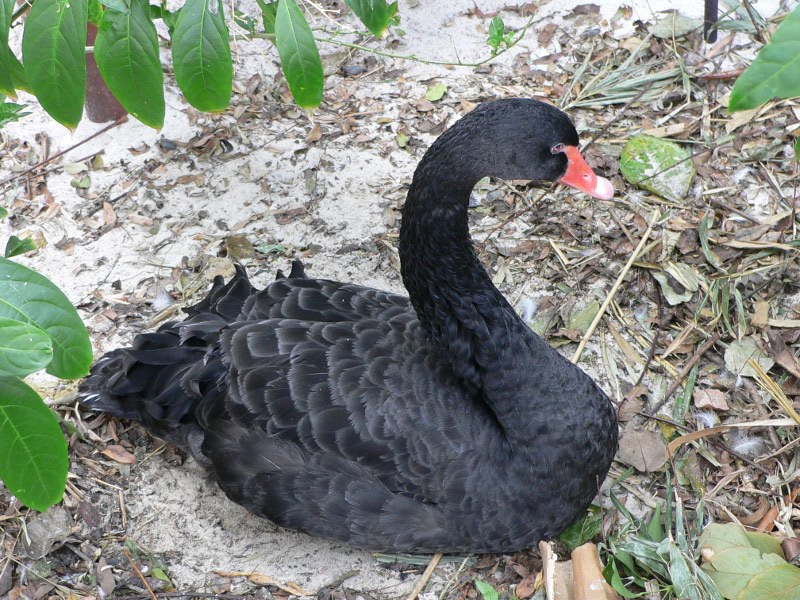
\includegraphics[width=8cm]{pictures/kuvitus/Cygnus_atratus1}
\end{center}
\bigskip

Aristoteleen tekemä jako deduktiivisiin ja induktiivisiin päättelyihin
ei ole enää nykypäivänä täysin toimiva.
Toisaalta tämä johtuu induktiopäättelyyn liittyvistä ongelmista,
toisaalta siitä, että esimerkiksi tilastollisia päättelymenetelmiä
ei ole helppo luokitella tällä tavoin.
Filosofiassa tutkitaan deduktion ja induktion lisäksi myös niin kutsuttuja
\termi{abduktiivinen päättely}{abduktiivisia} päättelyjä.
Lisämateriaalina olevassa kappaleessa 5.4 esitellään
\termi{matemaattinen induktio}{matemaattinen} eli
\termi{täydellinen induktio}{täydellinen induktio},
jota ei pidä sekoittaa filosofiassa esiintyvään induktiopäättelyyn.

Deduktiivista päättelyä on mahdollista soveltaa monenlaisissa tilanteissa.
Merkittävä deduktiivisen päättelyn sovellus on matemaattinen todistaminen,
jota tutkivaa logiikan osa-aluetta sanotaan joskus
\termi{matemaattinen logiikka}{matemaattiseksi logiikaksi} erotuksena
yleisemmin päättelyjä ja ajattelua tutkivasta
\termi{filosofinen logiikka}{filosofisesta logiikasta}.
Nykyään tärkeä logiikan sovelluskohde on tietotekniikka, joten logiikkaa
tutkitaan myös teoreettisen tietojen\-käsittely\-tieteen osana.
Tässä kurssissa keskitytään ensisijaisesti matemaattiseen logiikkaan.

\begin{esimerkki} Ovatko seuraavat päättelyt loogisesti päteviä? Perustele.
    \begin{enumerate}[a)]
        \item \kolmepaattely{Kaikki örjyt ovat nouvareita.}{Mikään surjimus ei ole nouvari.}{Mikään surjimus ei ole örjy.}
        \item \kolmepaattely{Kuusi on puu.}{Näre on puu.}{Näre on kuusi.}
        \item \kaksipaattely{Kaikki kohtaamani joulupukit ovat olleet tavallisia ihmisiä,
            \\& jotka ovat vain pukeutuneet joulupukiksi.}{Oikeaa joulupukkia ei ole olemassa.}
    \end{enumerate}
    \textbf{Ratkaisu:}
        \begin{enumerate}[a)]
            \item On. Jos jokin surjimus olisi örjy, niin silloin se oletuksen (1) nojalla olisi myös nouvari.
                Mutta oletuksen (2) mukaan mikään surjimus ei ole nouvari. Siis ei ole
                mahdollista, että jokin surjimus olisi örjy. 
            \item Ei. Vaikka kuusi ja näre ovat molemmat puita, niin ei siitä tarvitse seurata,
                että näre on kuusi. Itse asiassa näre tarkoittaa nuorta kuusta, mutta tämä on kielellinen sopimus.
                Logiikka ei suoraan ota kantaa sanojen merkityksiin.
                Vaikka väite on sinällään tosi, niin se ei seuraa oletuksista ja siksi päättely ei ole loogisesti pätevä.
            \item Ei. Kyseessä on induktiivinen päättely, joka ei ole loogisesti pätevä.
        \end{enumerate}
    \textbf{Vastaus:}
        a) on, b) ei, c) ei.
\end{esimerkki}

\begin{esimerkki}
    Ovatko seuraavat päättelyt loogisesti päteviä? Perustele.
    \begin{enumerate}[a)]
        \item Kaikki ajavat joskus ylinopeutta, joten pienestä lipsahduksesta ei tarvitse antaa rangaistusta.
        \item Pariisin tiedeakatemian professorit julistivat, että meteoriitteja ei ole olemassa,
            koska taivaalla ei ole kiviä.
            Siis meteoriitteja ei ole olemassa\footnote{Pariisin tiedeakatemia julisti vuonna 1772
            kuuluisan kemistin Lavoisier'n johdolla, että löydetyt meteoriitit ovat maanpäällisiä kiviä,
            joihin salama on iskenyt, ja kivien putoaminen taivaasta on fysikaalisesti mahdotonta.
            Vielä vuonna 1790 tiedemies Berthollet julisti Barbotaniin pudonneen meteoriitin olevan valitettava
            osoitus kansanuskomusten ja satujen kyvystä ottaa valtaansa kokonainen kaupunki.
            Nämä kriittiset kommentit johtivat siihen, että monet museot poistivat kokoelmistaan meteoriitteja 
            väärennöksinä.
            Vasta vuonna 1803 Jean-Baptiste Biot'n uraauurtava tutkimus L'Aiglen meteoriitista johti meteoriittien 
            alkuperän selviämiseen ja niiden yleiseen hyväksyntään tiedepiireissä.
            Lähde: Lindsay, E. M., Maskelyne and Meteors, Irish Astronomical Journal, vol. 8(3), p. 69, 1967.}.
        \item Lingvistiikan professori Miettisen mukaan Suomen voimassaolevat ravintoainesuositukset eivät perustu 
            uusimpiin tutkimustuloksiin.
            Ongelmia on erityisesti rasvojen käyttöä koskevissa suosituksissa.
            Siis Suomen nykyiset ravintoainesuositukset ovat vanhentuneet.
        \item Tunnettu pikkurikollinen Lipa Luihu nähtiin lauantai-iltana rautatieasemalla.
            Samana iltana varastettiin Urho Kestävän maastopyörä aseman pyörätelineestä.
            Siis Luihu oli varastanut Kestävän pyörän.
        \item Kolme prosenttia ihmisistä on nähnyt lentävän lautasen. Siis lentäviä lautasia on olemassa.
    \end{enumerate}
    \textbf{Ratkaisut:}
        \begin{enumerate}[a)]
            \item Kysymyksessä oleva päättely on virheellinen, koska se vetoaa sääntöjen rikkojien määrään eikä
                kyseisen rikkomuksen olosuhteisiin.
                Se, että useimmat ihmiset toimivat tai ajattelevat jollakin tavalla, ei logiikan mielessä todista
                mitään, koska enemmistö voi olla väärässä.
                
                Tätä päättelyvirhettä kutsutaan filosofiassa nimellä \termi{argumentum ad populum}{argumentum ad populum}
                eli vetoaminen lukumäärään.
                Yleisimmin se esiintyy yleiseen mielipiteeseen tai toimintatapaan vetoavissa johtopäätöksissä.
                Joskus vedotaan myös pienemmän mutta ylivertaisten joukon näkemykseen, esimerkiksi:
                ''Kaikki ne, jotka oikeasti osaavat ajaa autoa, ajavat joskus ylinopeutta.''
                Myös tämä päättely on virheellinen.
            \item Vaikkakin Pariisin tiedeakatemia edusti 1700-luvun parasta asiantuntemusta, myös asiantuntijat
                voivat olla väärässä.
                Lisäksi luonnontieteelliset tulokset eivät ole koskaan logiikan mielessä todistettuja ja mahdollisuus 
                virheeseen on suuri erityisesti uusien ja mullistavien löy\-dös\-ten kohdalla.
                
                Tieteellisessä menetelmässä kuitenkin pyritään siihen, että esitetyt väitteet ovat 
                \termi{falsifioituva}{falsifioituvia}.
                Ne voidaan kokeella tai havainnolla osoittaa vääräksi, kuten tässä tapauksessa tapahtuikin.
                Siksi tieteellinen tieto on itsensä korjaavaa ja lukuisissa koetilanteissa testattuja teorioita
                voidaan pitää käytännössä hyvin luotettavina, joten vetoaminen asiantuntijan näkemykseen on hyväksyttävää 
                argumentaatiota.
                Tällöin tulisi kuitenkin ensisijaisesti vedota asiantuntijoiden esittämiin perusteluihin eikä
                heidän asemaansa tai lukumääräänsä.
                Pelkästään useimpien asiantuntijoiden mielipiteeseen vetoava argumentti on tiukasti
                tulkittuna virhepäätelmä (katso a-kohta).
            \item Professori Miettinen ei ole ravitsemustieteen asiantuntija, joten hänen mielipidettään ei voida pitää 
                asiantuntijan näkemyksenä.
                Kysymyksessä on virheellinen argumentti, josta käytetään filosofiassa myös nimitystä
                \termi{argumentum ad verecundiam}{argumentum ad verecundiam} eli vetoaminen väärään auktoriteettiin.
                Lisäksi vetoaminen edes oikean asiantuntijan näkemykseen ei koskaan ole logiikan mielessä pätevä päättely.
            \item Päättely ei ole logiikan mielessä pätevä eikä myöskään hy\-väk\-syt\-tä\-vää argumentaatiota,
                koska  päättely perustuu ensisijaisesti Lipa Luihun henkilökohtaisiin ominaisuuksiin eikä itse
                rikokseen liittyviin havaintoihin. Tällaisesta päätelmästä käytetään filosofiassa nimitystä 
                \termi{argumentum ad hominem}{argumentum ad hominem} eli argumentoiminen henkilöä vastaan.
                
                Juridiikassa esimerkiksi tietoa henkilön aikaisemmasta rikoshistoriasta pidetään kuitenkin
                hyväksyttävänä aihetodisteena eli todisteena, jonka perusteella syyllisyyttä voidaan pitää
                todennäköisenä, vaikka se ei suoraan osoitakaan syyllisyyttä.
            \item Tämä päättely on logiikan mielessä pätevä, vaikka harvat asiantuntijat pitävät johtopäätöstä oikeana.
                Vika ei kuitenkaan ole päättelyssä vaan oletuksessa, jonka mukaan kolme prosenttia ihmisistä on nähnyt 
                lentävän lautasen.
                Tällaisia havaintoja ei voida pitää kovin luotettavina, koska ihmiset saattavat tehdä virheellisiä 
                havaintoja tai tarkoituksellisesti vääristellä totuutta.
        \end{enumerate}
    \textbf{Vastaukset:}
        a) ei, b) ei, c) ei, d), ei, e) on (varauksin).
\end{esimerkki}

\Harjoitustehtavat

\begin{enumerate}
    \item Onko päättely loogisesti pätevä? Perustele.
        \begin{enumerate}[a)]
            \item Kaikki ihmiset ovat kuolevaisia. Lasse-kissa on kuolevainen. Siis Lasse-kissa on ihminen.
            \item Kaikki koirat osaavat haukkua. Halli on koira. Siis Halli osaa haukkua.
        \end{enumerate}
    \item Ovatko seuraavat päättelyt loogisesti päteviä? Perustele.
        \begin{enumerate}[a)]
            \item \kolmepaattely{Kaikki tetraedrit ovat pyramideja.}{Jotkut kartiot ovat tetraedrejä.}
                {Jotkut kartiot ovat pyramideja.}
            \item \kolmepaattely{Kaikki sylinterit ovat lieriöitä.}{Mikään lieriö ei ole kartio.}
                {Jotkut sylinterit ovat kartioita.}
            \item \kolmepaattely{Luku $345$ päättyy numeroon $5$.}{Nollaan päättyvä luku on viidellä jaollinen.}
                {Luku $345$ on viidellä jaollinen.}
        \end{enumerate}
    \item Onko seuraava päättely loogisesti pätevä? Perustele.
        \begin{enumerate}[a)]
            \item Jos ulkona on pakkanen, menen hiihtämään. Ulkona ei ole pakkanen. Siis en mene hiihtämään.
            \item Jos ulkona on pakkanen, menen hiihtämään. En mene hiihtämään. Siis ulkona ei ole pakkanen.
            \item Jos tiedän nukkuvani, niin nukun. Jos tiedän nukkuvani, niin en nuku. Siis en tiedä nukkuvani.
        \end{enumerate}
    %\item Onko seuraava päättely loogisesti pätevä? Perustele.
    %    \neljapaattely{Kaikilla $x$ toteutuu $y$.}{Kaikilla $x$ toteutuu $z$.}{Jokin $x$ on olemassa.}
    %    {Joillakin $y$ toteutuu $z$.}
    \item Tutkitaan polynomia
        \[ P(x) = x^5 -10x^4+35x^3 -50 x^2 +25x. \]
        \begin{enumerate}[a)]
            \item Laske $P(0)$, $P(1)$, $P(2)$, $P(3)$ ja $P(4)$.
            \item Mitä voit sanoa luvuista $P(n)$, kun $n$ on luonnollinen luku?
            \item Testaa päätelmääsi kokeilemalla myös muilla luonnollisilla luvuilla esimerkiksi laskinta käyttäen.
        \end{enumerate}
    \item Arkiajattelussa käytetään usein ajattelumalleja, jotka eivät ole loogisesti perusteltavissa.
        Mikä virhe on seuraavissa päätelmissä?
        \begin{enumerate}[a)]
            \item Ilta-Sanomien kyselyssä $66\%$ vastaajista uskoo maan ulkopuoliseen elämään.
                Maan ulkopuolista elämää on olemassa.
            \item The Sunday Times -lehden haastattelussa kuuluisa tiedemies Stephen Hawking
                totesi pitävänsä lähes varmana, että avaruudessa on maan ulkopuolista älykästä elämää.
                Maan ulkopuolista elämää on olemassa.
            \item Tiedemiehistä 90\% väittää, että nykyinen ilmastonmuutos on ihmisen aiheuttamaa
                eikä johdu maapallon lämpötilan luontaisesta jaksollisuudesta.
                Siis nykyinen ilmastonmuutos on ihmisen aiheuttamaa.
            \item Televisiouutisissa kerrottiin, että toisen maailmansodan aikainen holokausti oli
                vain liittoutuneiden propagandaa.
                Siis holokaustia ei tapahtunut toisen maailmansodan aikana.
            %\item Vuonna 2079, kaksi vuotta kvanttiaaltoihin pohjaavan kommunikaatiomenetelmän keksimisen jälkeen,
            %    tiedemiehet havaitsevat noin 170 valovuoden päässä sijaitsevan kehittyneen sivilisaation
            %    tietoliikenteestä aiheutuvia signaaleja.
            %    Siis ufo-havaintoihin uskoneet ovat olleet koko ajan oikeassa.
        \end{enumerate}
    \item Ovatko seuraavat päättelyt loogisesti päteviä? Perustele.
        \begin{enumerate}[a)]
            \item \kolmepaattely{Kaikilla $x$ toteutuu $y$.}{Joillakin $z$ toteutuu $x$.}{Joillakin $z$ toteutuu $y$.}
            \item \kolmepaattely{Kaikilla $A$ toteutuu $B$.}{$C$ toteuttaa $B$:n.}{$C$ toteuttaa $A$:n.}
            \item \kolmepaattely{Kaikilla $A$ toteutuu $B$.}{Millään $C$ ei toteudu $B$.}{Millään $C$ ei toteudu $A$.}
        \end{enumerate}
\end{enumerate}

\subsection*{Kotitehtäviä}

\begin{enumerate}
    \item Ovatko seuraavat päättelyt päteviä? Perustele.
        \begin{enumerate}[a)]
            \item \kolmepaattely{Kaikki kissat osaavat kehrätä.}{Tämä eläin osaa kehrätä.}{Tämä eläin on kissa.}
            \item \kolmepaattely{Kukaan laiska opiskelija ei selviä kokeesta.}
                {On opiskelijoita, jotka selviävät kokeesta.}{On opiskelijoita, jotka eivät ole laiskoja.}
        \end{enumerate}
    \item Ovatko seuraavat päättelyt päteviä? Perustele.
        \begin{enumerate}[a)]
            \item \kolmepaattely{Neljäkkään lävistäjät ovat kohtisuorassa toisiaan vastaan.}
                {Neljäkäs on suunnikas.}{Suunnikkaan lävistäjät ovat kohtisuorassa toisiaan vastaan.}
            \item \kolmepaattely{Kaikki suorakulmiot ovat suunnikkaita.}{Jotkut nelikulmiot ovat suorakulmioita.}
                {Jotkut nelikulmiot ovat suunnikkaita.}
            \item \kolmepaattely{Kolmio $ABC$ on tasakylkinen.}{Tasasivuiset kolmiot ovat tasakylkisiä.}
                {Kolmio $ABC$ on tasasivuinen.}
        \end{enumerate}
    \item Ovatko seuraavat päättelyt päteviä? Perustele.
        \begin{enumerate}[a)]
            \item \kaksipaattely{Kaikki lammasfarmin lampaat ovat joko mustia tai valkoisia.}
                {Kaikki lampaat ovat mustia tai valkoisia.}
            \item \neljapaattely{Tavallisessa korttipakassa kortti on aina joko pata,\\& risti, hertta tai ruutu.}
                {Pata- ja risti-kortit ovat mustia.}{Hertta- ja ruutu-kortit ovat punaisia.}
                {Kaikki tavallisten korttipakkojen kortit ovat\\ & joko mustia tai punaisia.}
        \end{enumerate}
    %\item Onko seuraava päättely pätevä? Perustele.
    %    \neljapaattely{Millään $x$ ei toteudu $y$.}{Kaikilla $x$ toteutuu $z$.}{Jokin $x$ on olemassa.}
    %    {Joillakin $z$ ei toteudu $y$.}
    \item Jäämaa on kokonaan Merimaan itäpuolella.
        Kummallakin on etelärajaa Aurinkomaan kanssa.
        Merimaalla ja Aurinkomaalla on länsiraja Lumimaan kanssa.
        Kukkamaa on kokonaan Jäämaan ja Aurinkomaan itäpuolella.
        \begin{enumerate}[a)]
            \item Onko Merimaalla ja Kukkamaalla yhteistä rajaa?
            \item Voiko Lumimaalla ja Kukkamaalla olla yhteistä rajaa?
        \end{enumerate}
    \item Ovatko seuraavat päättelyt päteviä? Perustele.
        \begin{enumerate}[a)]
            \item \kolmepaattely{Millään $x$ ei toteudu $y$.}{Kaikilla $z$ toteutuu $x$.}{Millään $z$ ei toteudu $y$.}
            \item \kolmepaattely{Kaikilla $A$ toteutuu $B$.}{Joillakin $C$ toteutuu $B$.}{Joillakin $A$ toteutuu $C$.}
        \end{enumerate}
\end{enumerate}
